\documentclass[conference]{IEEEtran}
\IEEEoverridecommandlockouts
% The preceding line is only needed to identify funding in the first footnote. If that is unneeded, please comment it out.
\usepackage{cite}
\usepackage{amsmath,amssymb,amsfonts}
\usepackage{algorithmic}
\usepackage{graphicx}
\usepackage{textcomp}
\usepackage[table]{xcolor}
\usepackage{longtable}
\usepackage{array}
\usepackage[german]{babel}
\usepackage[utf8x]{inputenc}
\usepackage[german=quotes]{csquotes}
\usepackage{url}
\def\BibTeX{{\rm B\kern-.05em{\sc i\kern-.025em b}\kern-.08em
    T\kern-.1667em\lower.7ex\hbox{E}\kern-.125emX}}
\begin{document}

\title{Random Forest und k-Nearest-Neighbour für die Detektion von Schreibstiländerungen zur Autorenzuordnung}





\author{\IEEEauthorblockN{Engler, Rebecca; Fandrich, Anna; Gühler, Tobias; Mitterlehner, Johanna; Schilling, Anabel;\\ Wittmann, Clarissa; Wutke, Leon}
\IEEEauthorblockA{Fakultät CB} \\
\textit{HS Mittweida}
}
\maketitle

\begin{abstract}
In diesem Paper wird der Ansatz vorgestellt, die Detektion von unterschiedlichen Autoren geschriebener Textsequenzen innerhalb eines Dokuments, anhand von Änderungen im Schreibstil zu detektieren. Die Frage nach der Existenz von mehr als nur einem Autor innerhalb eines Dokuments wird mit k-Nearest-Neighbour-Klassifikation beantwortet und die genaue Detektion der Position jedes Autors erfolgt mit Hilfe eines Random-Forest-Klassifikators. Dabei wird jeder Absatz des Textes von einer Ansammlung stilometrischer Eigenschaften repräsentiert. Diese werden anschließend den Algorithmen übergeben. Dieser Ansatz wurde gewählt, um stilometrische Features den Worteinbettungen des State of the Art Modells gegenüberzustellen. Bei der Auswertung des Random-Forest-Klassifikators, wurde eine leichte Verbesserung, von 0.004, gegenüber dem Micro-Average-F1-Score des State of the Art erreicht. Der Macro-Average-F1-Score des kNN fällt hier schlechter aus als der des State of the Art Modells. Der Wert zur Detektion für nur einen Autor innerhalb eines Dokuments liegt allerdings bei 0.7, was für die Beantwortung der Frage, ob ein Dokument von nur einem Autor geschrieben wurde, ausreicht. Alle hier zur Klassifikation verwendeten Codes und Dateien, mit Ausnahme der antrainierten Modelle werden öffentlich gemacht und sind unter folgendem Link \url{https://github.com/1d438ef6/Authorship-Detection} zu finden.

\end{abstract}

\begin{IEEEkeywords}
	machine learning, text mining, author detection, random forest, kNN
\end{IEEEkeywords}

\section{Einleitung}
	Schreibstiländerungsdetektion ist ein Verfahren, dessen Ziel es ist, zu bestimmen, wo in einem gemeinschaftlich geschriebenen Text ein Wechsel des Autors stattfindet \cite{e_b1}. Es überprüft, wie gleichmäßig der Schreibstil im ganzen Text ist und an welchen Stellen er sich ändert, was auf einen Wechsel des Autors hindeutet \cite{e_b2}. Dabei werden verschiedene stilistische Eigenschaften, sogenannte Features, verwendet. Diese werden im ganzen Text miteinander verglichen und somit überprüft, an welchen Stellen sich wie viele Features wie stark verändern, um einzuschätzen, ob ein Autorenwechsel stattgefunden hat \cite{e_b3}. Das Verfahren kann für verschiedene forensische Zwecke verwendet werden, wie zum Beispiel die Identifizierung von Plagiaten \cite{e_b2}.
	
	
	Die Aufgabe hierbei besteht darin, in einem Dokument, geschrieben von mehreren Autoren, Änderungen des Schreibstils und den damit verbundenen Wechsel des Autors zu erkennen. Dafür wird angenommen, dass der Wechsel des Stils den Wechsel des Autors impliziert. Gegeben sind hierfür englische Dokumente. Diese können bis zu zehn Stiländerungen enthalten und von höchstens drei Verfassern stammen. Gleichzeitig können Änderungen des Stils nur zwischen Absätzen vorkommen, was einen Autor und einen Stil pro Absatz impliziert. Diese festgesetzten Bedingungen sind für die Aufgabenlösung unabdingbar.
	
	\begin{figure}[h]
		\centering
		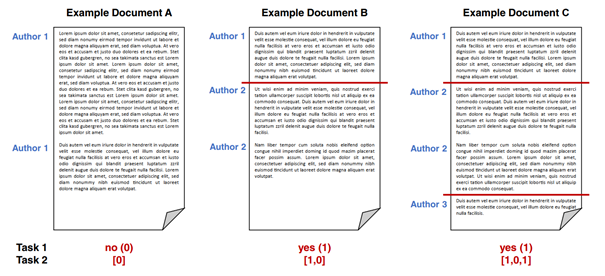
\includegraphics[width=0.9\linewidth]{Aufgabenbeschreibung}
		\caption{Beispieldokumente, die Stiländerungmuster darstellen und die erwarteten Lösungen für  Aufgabe 1 (ein oder mehrere Autoren) und Aufgabe 2 (Position der Stiländerungen).\cite{e_b4}}
		\label{fig:aufgabe}
	\end{figure}
	
	Zur Aufgabenlösung wird der Vorgang der Stiländerungsdetektion in zwei Teilaufgaben aufgeteilt. Die erste Aufgabe soll die Frage beantworten, ob ein Dokument von einem oder mehreren Autoren geschrieben wurde. In der zweiten Aufgabe soll bestimmt werden, zwischen welchen aufeinanderfolgenden Absätzen eine Schreibstiländerung und somit auch ein Autorenwechsel stattfand. Diese beiden Teilaufgaben und die jeweils für diese erwarteten Ausgaben werden in Abbildung \ref{fig:aufgabe} nochmals verdeutlicht. Dokument A enthält keine Schreibstiländerungen und wurde somit von nur einem Autor verfasst. Dokument B enthält eine einzelne Stiländerung zwischen Absatz eins und zwei, während Dokument C zwei Stiländerungen aufzeigt. 
	
	Ziel des Projektes ist es also, mithilfe eines Programms und maschinellen Lernverfahren zu ermitteln, ob die bereitgestellten Dokumente, welche aus Stackoverflow extrahiert wurden, Änderungen des Stils enthalten. Trifft dies zu wird versucht, diese Änderungen im Text zu lokalisieren.
	
	
	Im Folgenden werden verwandte Werke besprochen. Daraufhin wird sich mit den Methoden, bestehend aus Datensatz, Algorithmus und Features beschäftigt. Abschließend werden die Ergebnisse dargelegt, woraufhin die Diskussion sowie Arbeitsansätze für die Zukunft und ein Fazit folgen.
	
\section{Verwandte Werke}
Seit dem Jahr 2017 erscheint \textit{\enquote{Style Change Detection}} als Aufgabe des PAN als Teil des CLEFs (Conference and Labs of the Evaluation Forum). Seitdem wurden zahlreiche Vorgehen erprobt, um die Aufgabenstellung zu bewältigen und die bisherigen Ergebnisse zu verbessern. \cite{vw_b1} 

Iyer und Vosoughi \cite{vw_b2} nutzen Googles BERT-Modell für die Erstellung von Worteinbettungen auf Satzebene als Repräsentation der Texte. Mit den Ausgaben aus BERT wird eine Feature-Matrix erstellt, die dann für aufeinanderfolgende Absätze und das gesamte Dokument zusammengefasst wird. Zuletzt erfolgt die Übergabe an einen Random Forest Klassifikator zum Training. Da dieses Paper beim PAN 2020 die besten Ergebnisse erzielt hat, wird es im Rahmen dieser Arbeit als State of the Art Modell betrachtet und als Baseline zur Beurteilung der Ergebnisse genutzt.

Singh et al. \cite{vw_b3} extrahieren Eigenschaften zweier Absätze und stellen diese als Eigenschaftsvektoren dar. Anhand der Unterschiede dieser zwei Vektoren und eines Klassifikators für Logistische Regression wird die Stiländerungserkennung durchgeführt. 

Deibel und Löfflad \cite{vw_b4} kombinieren Worteinbettungen mit bekannten stilometrischen Eigenschaften. Sie nutzen ein Multi-Layer-Perceptron zur Erkennung multipler Autoren im Dokument und ein bidirektionales Long short-term memory (LSTM) zur Erkennung der Stiländerung. Dieser Ansatz iteriert nachfolgend und teilt unter Zuhilfenahme eines Attribution-Algorithmus einen Autor pro Absatz zu.

Viele der bisherigen Vorgehen extrahieren stilometrische Eigenschaften aus den vorgegebenen Textdaten und nutzen diese, um Ähnlichkeit zwischen den Absätzen festzustellen \cite{vw_b5,vw_b6,vw_b7}. Der in der vorliegenden Arbeit verwendete Ansatz ähnelt diesem Muster. Unterschiede sind unter anderem bei der Verarbeitung der Features anzumerken. 

Wie Deibel und Löfflad \cite{vw_b4} in ihrer Arbeit anmerken, scheint die Auswahl der verwendeten Features großen Einfluss auf das Endergebnis der Style-Change-Detection-Aufgabe zu haben. So erzielten sie auch mit lediglich fünf Eigenschaften gute Ergebnisse auf dem in ihrer Arbeit verwendeten Datensatz.  

In der vorliegenden Arbeit wurde hier angesetzt und nur Features verwendet, die aussagekräftig für die Problemlösung waren. 

Singh et al. \cite{vw_b8} diskutieren die Problematik, dass extrahierte Eigenschaften bei kurzen Dokumenten- bzw. Absatzlängen weniger relevante stilometrische Information bieten. Sie nutzten daher kompakte Feature-Sets, die mit dem Stil zusammenhängende Features über das gesamte Dokument sammeln.
  

Neben der Verwendung bekannter stilometrischer Eigenschaften wurden in verwandten Werken auch Worteinbettungen als textuelle Eigenschaften auf Wort- \cite{vw_b9} und Satzebene \cite{vw_b2} zur Autorenzuordnung eingesetzt. Auf die Nutzung dieser wird bei der vorliegenden Arbeit verzichtet.


\section{Methoden}
	\subsection{Datensatz}
		Zur Lösung des in der Einleitung beschriebenen Problems liegen ein Traningsdatensatz sowie ein Validierungsdatensatz vor. Weiterhin sind beide Datensätze unterteilt in je einen wide sowie einen narrow Datensatz. Der narrow Datensatz ist auf einen kleinen Themenbereich beschränkt, während der wide Datensatz einen größeren Themenbereich umfasst. Die Anzahl der Dokumente, die in jedem der Datensätze enthalten sind, lässt sich aus Tabelle \ref{tab:ds_1} entnehmen.
		
		\begin{table}[htbp]
			\caption{Verteilung der Autorenanzahl über die gegebenen Datensätze}
			\begin{center}
				\begin{tabular}{|c|c|c|c|c|}
					\hline
					 & 1 Autor & 2 Autoren & 3 Autoren & Gesamt \\
					\hline
					Training-narrow & 1709 & 853 & 855 & 3417 \\
					\hline 
					Training-wide & 4024 & 1990 & 2015 & 8029 \\
					\hline
					Validation-narrow & 854 & 415 & 443 & 1442\\
					\hline 
					Validation-wide & 863 & 420 & 430 & 1713\\
					\hline
				\end{tabular}
				\label{tab:ds_1}
			\end{center}
		\end{table}
	
		
		Für die gegebenen Daten wurde zunächst eine Datenexploration ausgeführt, um deren Struktur zu analysieren. Hierbei wurde anfangs die Verteilung der Autoren über die Dokumente aller Datensätze betrachtet. Dabei stellte sich heraus, dass ein Autor in etwa doppelt so oft vorkommt wie zwei oder drei Autoren. Die genaue Aufschlüsselung der Autorenanzahl in jedem Datensatz findet sich in Tabelle \ref{tab:ds_1}. Daher lässt sich vermuten, dass ein Autor am besten klassifizierbar ist, da dafür am meisten Daten zum Training vorhanden sind.
		
		Im nächsten Schritt wurde analysiert, ob die Dokumente Code enthalten, welcher bei der Erstellung der Dokumente mit aus den Stackoverflow Seiten extrahiert wurde. Der gefundene Code wurde dann entfernt, da dieser, aufgrund der vorgegebenen Syntaktik, meist andere autorspezifische Merkmale aufweist als natürliche Sprache (in Textform).
		Obwohl vorgegeben war, dass alle Dokumente in englischer Sprache verfasst wurden, wurde als letztes die Sprache der gegebenen Dokumente untersucht, um anderssprachige Dokumente aus dem Datensatz auszuschließen. Dabei wurden Bruchstücke deutscher Sprache und Sprachen aus dem asiatischen Raum gefunden.
		
\subsection{Klassifikationsmodell}
	
	\begin{figure}[h]
		\centering
		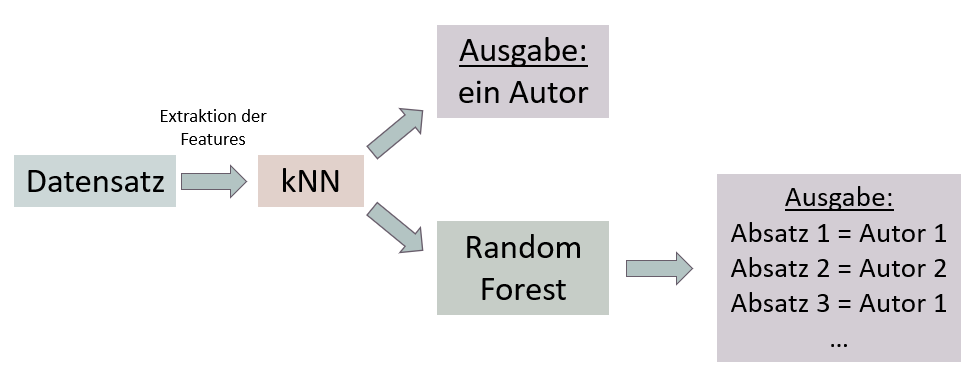
\includegraphics[width=0.8\linewidth]{alg}
		\caption{Schematische Darstellung des hier vorgestellten zwei Komponentensystems zur Autorenklassifikation}
		\label{fig:algorithm}
	\end{figure}
	
	
	In Aufgabe 1 soll festgestellt werden, ob das Dokument von mehreren Autoren verfasst wird, ohne dass die Position des Wechsels ermittelt werden muss. Hierfür wird davon ausgegangen, dass die Features, über das komplette Dokument berechnet, sich unterscheiden, wenn nur einer oder mehrere Autoren an einem Dokument beteiligt sind. Dafür wird ein kNN-Klassifikator aus der sklearn-Bibliothek \cite{ma_b1} von Python verwendet. Als Eingabe werden die Features genutzt, die über jedes Dokument berechnet werden. Der kNN wird mit dem Trainingsdatensatz trainiert, bevor der Validierungsdatensatz zum validieren genutzt wird. Hierfür wird die Anzahl der Nachbarn mit $k=200$ gewählt, welche durch Testläufe ermittelt wurde. Die Anzahl der Klassen ist gleich der Anzahl an möglichen Autoren in einem Dokument. 
	KNN bietet dabei die Möglichkeit, Dokumente mit nur einem Autor schnell auszusortieren. Somit lässt sich der mit Random-Forest-Klassifikator noch zu klassifizierende Datensatz erheblich reduzieren.
	
	
	Für Aufgabe 2, also um zu erkennen, welcher Autor den jeweiligen Absatz geschrieben hat beziehungsweise zwischen welchen Absätzen eine Stiländerung stattgefunden hat, wird ein Random-Forest-Klassifikator, der scikit-learn Bibliothek für Python \cite{ma_b1}, mit verschiedenen Features genutzt. Auf die verwendeten Features wird im nächsten Abschnitt eingegangen. Diese Features werden über jeden einzelnen Absatz berechnet. Die Featurerepräsentation wird schließlich an den Random-Forest-Klassifikator übergeben, der die Absätze dann wie nachfolgend beziehungsweise in Abbildung \ref{fig:rfcalgorithm} erklärt den Autoren zuordnet.
	
	Der Ablauf der Autorenklassifikation, sowie das Zusammenspiel der beiden genutzten Klassifikatoren, wird in Abbildung \ref{fig:algorithm} schematisch dargestellt.
	
	Random-Forest-Klassifikatoren haben einige Vorteile, die für die Aufgabe nützlich sind. Unter anderem sind Training sowie Voraussage schnell. Der Algorithmus kann zudem parallel implementiert werden und ist für hochdimensionale Probleme – wie Stiländerungsdetektion – geeignet. \cite{ma_b2} Außerdem nutzt er nicht alle Daten, sodass ein ausreichend großer Evaluationsdatensatz vorhanden ist.
	
	Die Anzahl der Entscheidungsbäume, die ein Random-Forest-Klassifikator nutzt, kann variieren. Es hat sich aber gezeigt, dass eine höhere Anzahl an Bäumen nicht zwingend bessere Ergebnisse liefert. Da der Random-Forest-Klassifikator mehrere Entscheidungsbäume auf einmal verwendet, ist auch die Gefahr des Overfittings reduziert. \cite{ma_b2}
	
	\begin{figure}[h]
		\centering
		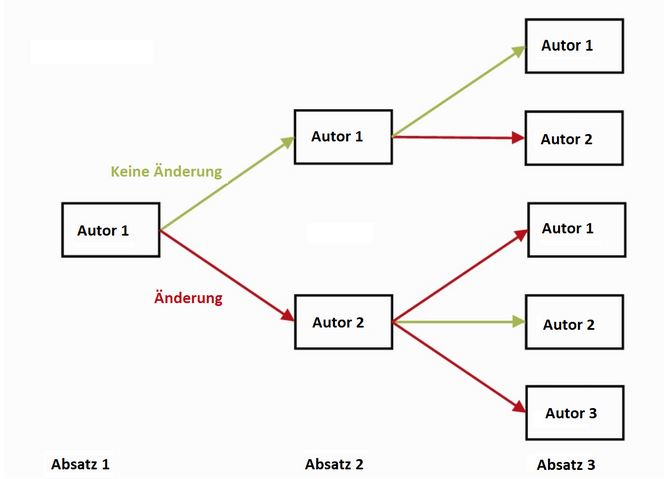
\includegraphics[width=0.7\linewidth]{Unbenannt}
		\caption{Schematische Darstellung der Autorenzuordnung}
		\label{fig:rfcalgorithm}
	\end{figure}
	
	
	Da ein Autorenwechsel nur zwischen den Absätzen stattfindet, kann angenommen werden, dass der erste Absatz von Autor 1 geschrieben wurde. Wird eine Änderung zu Absatz 2 festgestellt, dann wurde dieser Absatz von einem anderen Autor (Autor 2) geschrieben, andernfalls wurde auch dieser Absatz von Autor 1 verfasst. Das wird durch das gesamte Dokument fortgeführt, wobei der dritte Absatz auch von Autor 3  geschrieben worden sein kann. Die Voraussetzung ist allerdings, dass es in Absatz 2 einen Autorenwechsel von Autor 1 zu Autor 2 gibt. Um einen dritten Autor festzustellen, werden beispielsweise Absatz 1 und Absatz 3 miteinander verglichen, um zu bestimmen, ob zwischen diesen beiden Absätzen ein Autorenwechsel stattgefunden hat. Wenn es eine Änderung gab, wurde Absatz 3 von Autor 3 geschrieben, ansonsten wieder von Autor 1. Das kann man Abbildung \ref{fig:rfcalgorithm} entnehmen. 
	
	Während des gesamten zuvor beschriebenen Prozesses werden alle Featuresets, die einen Autor beschreiben gemittelt, da zwei Absätze, die den gleichen Autor beschreiben eine leichte Variation der Features aufweisen. Die gemittelten Featuresets werden ab dem dritten Absatz als Referenz benötigt, um eine Autorenzuordnung möglich zu machen.
	
\subsection{Features}
	Autoren können anhand von stilometrischen Features unterschieden werden. Es gibt vier Arten von solchen Features: lexikalische, syntaktische, strukturelle und inhaltsbasierte. In Tabelle \ref{tab:features} ist eine Auswahl der verwendeten Features gelistet. Es wurden hauptsächlich lexikalische Features verwendet, da sie zeigen, welche Satzzeichen und Wörter Autoren unabhängig von anderen Faktoren verwenden \cite{mf_b1}.
	 
	Um eine allgemeine Unterscheidung von Autoren zu erhalten, sollte der Ansatz nicht auf inhaltsbasierten Features aufbauen, da der Gebrauch der Wörter meist vom Inhalt abhängt und somit je nach Inhalt eines Textes stark variiert. Diese Features sind für die gegebene Aufgabe nicht optimal und weitestgehend unbrauchbar \cite{mf_b2}.
	Außerdem eignen stilometrische Features sich gut für längere Texte anstelle von kurzen Nachrichten, wie z.B. Tweets, und sind somit gut für das gegebene Datenset geeignet \cite{mf_b3}.
	
	Nachfolgend wird eine Auswahl der Features aus Tabelle \ref{tab:features} erklärt:
	
	Ein wichtiges Feature ist der Flesch Reading Ease. Diese Formel berechnet die Lesbarkeit des Textes und bestimmt somit die Schulbildung, die der Autor benötigt hat, um den Text zu schreiben. Sie hängt von verschiedenen Faktoren ab:
	
	\bigskip
	$RE = 206.835 - 84.6*WL - 1.015*SL$ \cite{mf_b7}
	\bigskip
	
	$WL$ repräsentiert hierbei die durchschnittliche Wortlänge in Silben, $SL$ die durchschnittliche Satzlänge. Die in der Formel vorkommenden Zahlen basieren auf Erkenntnissen der Lesbarkeitsforschung und den statistischen Häufigkeiten von Silbenlänge, Wortlänge und Satzlänge im Englischen \cite{mf_b4}. \newline 
	Die Anzahl an Füllwörtern ist ebenfalls ein diskriminierendes Feature, da die Anzahl an Synsemantika je nach Autor zwischen 150 und 675 verschiedenen Wörtern liegen kann. Synsemantika sind Wörter mit geringer inhaltlicher Bedeutung, die aber grammatikalisch wichtig sind. Ein Beispiel wäre das Wort ‘dieser’. \cite{mf_b5}
	
	Die folgenden drei Features wurden selbst entwickelt und wurden ohne Referenzliteratur in das hier vorgestellte Modell implementiert:
	
	Die Satzkomplexität ist ein Maß dafür, wie komplex ein Autor seine Sätze gestaltet. Dabei wird die Anzahl der im Absatz vorhandenen Kommata durch die Anzahl an Sätzen im entsprechenden Absatz geteilt. Anschließend wird dieser Wert noch auf die Anzahl aller Sonderzeichen im Text gewichtet. Der daraus entstehende Wert diskriminiert den Autor stark. \newline Ein ebenfalls gut funktionierendes Feature stellt die Wortvarianz dar. Sie ist ein Maß für die Anzahl verschiedener Wörter in einem Text. Dabei wird diese auf die Textlänge gewichtet. Dabei sind die Wörter nicht lemmatisiert. \newline Das vermutlich am stärksten diskriminierende Feature aus Tabelle \ref{tab:features} ist das \textit{Random-Forest-Feature}. Bei diesem Feature handelt es sich um eine Vorhersage, welcher Autor dem Absatz zuzuordnen ist. Diese Vorhersage stammt von einem mit allen anderen Features antrainierten Random-Forest-Klassifikator. Dieses Modell hat eine Genauigkeit von ca. 70 Prozent.
	
	\begin{table}[htbp]
		\caption{ Zur Detektion der Schreibstiländerungen verwendete stilometrische Features, sortiert nach ihrer Art}
		\begin{center}
			\begin{tabular}{|p{4cm}|p{3cm}|}
				\hline
				\multicolumn{2}{|l|}{\textbf{1.1 Lexikalisch-wortbasierte Features}} \\
				\hline 
				Absolute Zahl an Wörtern & Die absolute Anzahl an Wörtern pro Absatz \\
				\hline
				Relative Anzahl an kurzen Wörtern  & Wörter mit 1-3 Zeichen, relativ zur Absatzlänge \\
				\hline 
				Relative Satzlänge & Die Satzlänge, relativ zur Satzanzahl \\
				\hline
				Silben pro Wort \cite{silben} & Die durchschnittliche Anzahl an Silben pro Wort \\
				\hline
				Flesch Reading Ease & Genaue Beschreibung im Text\\
				\hline
				Relative Worthäufigkeit & Die Worthäufigkeit, relativ zur Absatzlänge \\
				\hline
				Wortvarianz & Genaue Beschreibung im Text\\
				\hline
				\multicolumn{2}{|l|}{\textbf{1.2 Lexikalisch-zeichenbasierte Features}} \\
				\hline
				Relative Anzahl von Abkürzungen mit Sonderzeichen ‘ (zur Absatzlänge) & Beispiel: I’m, you’re, c’mon \\
				\hline
				Satzkomplexität & Genaue Beschreibung im Text \\
				\hline
				\multicolumn{2}{|l|}{\textbf{2. Syntaktische Features}} \\
				\hline
				Relative Anzahl an Füllwörtern & Beispiel: 'of','is','the' \\
				\hline
				\multicolumn{2}{|l|}{\textbf{3. Strukturelle Eigenschaften}} \\
				\hline
				Satzanzahl & Die Anzahl der Sätze pro Absatz \\
				\hline 
				Wortzahl & Die durchschnittliche Anzahl an Wörtern pro Satz \\
				\hline
				\multicolumn{2}{|l|}{\textbf{4. Sonstige Features}} \\
				\hline
				Random-Forest-Feature & Genaue Beschreibung im Text \\
				\hline
				Sprache \cite{mf_b6} & Im Text vorkommende nicht-englische Textsegmente \\
				\hline
			\end{tabular}
			\label{tab:features}
		\end{center}
	\end{table}
\section{Ergebnisse}
	Im Rahmen der ersten Aufgabe wurde die Anzahl der Autoren, welche ein Dokument verfasst haben, klassifiziert. Um den hier vorgestellten Ansatz, die Detektion der Autoren mittels kNN auf Dokumentenlevel, zu evaluieren, wurden beide zur Verfügung gestellten Datensätze verwendet. Hierfür wurden die F1-Scores für jeden Datensatz einzeln berechnet. Diese F1-Scores wurden dann klassenweise über die beiden Datensätze gemittelt. Um eine bessere Vergleichbarkeit der Ergebnisse zu erreichen, wurde am Ende noch der Macro-Average-F1-Score über alle Klassen berechnet. Die Ergebnisse der Evaluation sind in Tabelle \ref{tab:erg1} dargestellt. Tabelle \ref{tab:erg2} zeigt den erreichten Macro-Average-F1-Score des hier vorgestellten Modells sowie den Average-F1-Score des State of the Art Modells. Da in der Arbeit von Iyer und Vosoughi kein Macro-Average-F1 berechnet wurde, wird zum Vergleich der Average-F1-Score aus deren Veröffentlichung genutzt.
	
	\begin{table}[htbp]
		\caption{Ergebnisse der Autorenklassifikation mittels kNN auf Dokumentenlevel für jede Klasse }
		\begin{center}
			\begin{tabular}{|c|c|c|c|}
				\hline
				 & \multicolumn{3}{|c|}{\textbf{Anzahl Autoren}} \tabularnewline
				\hline
				 & 1 & 2 & 3 \\
				 \hline
				 \textbf{gemittelte F1-Scores} & 0,7 & 0,045 & 0,41 \\
				 \hline
			\end{tabular}
			\label{tab:erg1}
		\end{center}
	\end{table}
	\begin{table}[htbp]
		\caption{Gemittelte Ergebnisse der Autorenklassifikation auf Dokumentenlevel von dem hier vorgestellten Modell sowie dem State of the Art Modell}
		\begin{center}
			\begin{tabular}{|ccc|}
				\hline
				& \textbf{Macro-Average-F1} & \textbf{Average-F1} \\
				\cellcolor{gray!15}\textbf{Engler(2022)} & \cellcolor{gray!15}0,385 & \cellcolor{gray!15} --- \\
				\textbf{State of the Art} & --- & 0,856 \\
				\hline
			\end{tabular}
			\label{tab:erg2}
		\end{center}
	\end{table}
	
	Im Rahmen der zweiten Aufgabe sollte für die Dokumente, welche von mehreren Autoren verfasst wurden, festgestellt werden, zwischen welchen Absätzen der Autorenwechsel stattfindet. Auch hierfür wurden zur Evaluation des hier vorgestellten Modells, welches einen Random-Forest-Klassifikator auf Absatzlevel nutzt, beide Datensätze ausgewertet. Hierfür wurde zunächst für beide Datensätze der Micro-Average-F1-Score berechnet. Anschließend wurde der Micro-Average-F1-Score über beide Datensätze gemittelt. Die Ergebnisse der Evaluation sind in Tabelle \ref{tab:erg3} dargestellt.
	
	\begin{table}[htbp]
		\caption{Ergebnisse der Autorenklassifikation mittels Random Forest auf Absatzlevel inklusive Vergleich zum momentanen State of the Art von Iyer und Vosoughi}
		\begin{center}
			\begin{tabular}{|lc|}
				\hline
				 & \textbf{Micro-Average-F1} \\
				 \cellcolor{gray!15}\textbf{Engler(2022)} & \cellcolor{gray!15}0,859 \\
				 \textbf{State of the Art} & 0,856 \\
				\hline
			\end{tabular}
			\label{tab:erg3}
		\end{center}
	\end{table}
\section{Diskussion}
	Vergleicht man für die erste Aufgabe den Macro-Average-F1-Score des hier vorgestellten Modells im Gegensatz zum Average-F1-Score des State of the Art Modells fällt zunächst auf, dass das hier vorgestellte Modell schlechter abschneidet. Dieser niedrige Wert erklärt sich dadurch, dass das hier vorgestellte Modell bei Dokumenten, welche von mehreren Autoren geschrieben wurden, nicht optimal differenzieren kann, ob das Dokument nun von zwei oder drei Autoren verfasst wurde. Allerdings zeigt sich, dass die Klassifikation von Dokumenten, welche nur einen Autor haben, stabil möglich ist. Dies ist für das Modell vollkommen ausreichend, da es als Zweikomponentensystem aufgebaut ist. Im ersten Schritt wird nur klassifiziert, ob ein Dokument mehrere Autoren hat oder nicht. Wie viele Autoren ein Dokument genau hat ist, erst einmal irrelevant. Im zweiten Schritt werden dann die Dokumente mit mehreren Autoren weiterverarbeitet. Durch diese Art der Datenverarbeitung reduziert sich die Größe des Datensatzes, da Dokumente, welche von nur einem Autor geschrieben wurden, nicht weiterverarbeitet werden müssen.
	
	
	
	Vergleicht man den aktuellen State of the Art mit dem hier vorgestellten Modell fällt auf, dass das vorgestellte Modell eine minimal bessere Klassifikation erreicht. Eine Erklärung hierfür könnte sein, dass das vorgestellte Modell das Problem der Autorenklassifizierung leicht abstrahiert, um eine leichtere Klassifikation zu ermöglichen. Während Iyer und Vousoughi mithilfe eines Random-Forest-Klassifikators direkt klassifizieren, welcher Autor welchem Absatz zuzuordnen ist, klassifiziert das hier vorgestellte Modell, ob zwischen den Absätzen ein Autorenwechsel stattgefunden hat. Der Autor wird dann über den Wechsel bestimmt, wobei zur Vereinfachung die Annahme getroffen wird, dass Absatz eins auch immer von Autor eins geschrieben wurde. Da es jedoch in den gelabelten Validierungsdatensätzen auch Dokumente gibt, in denen der erste Absatz nicht von Autor eins geschrieben wurde, führt dies zu als falsch gekennzeichneten, aber dennoch richtig klassifizierten Dateien. Ein weitere Problematik wird dadurch eingeführt, dass jedem Klassifikationsvorgang Fehler innewohnen. Da in dem hier vorgestellten Modell für jeden Absatz eine Klassifikation durchgeführt wird, potenziert sich die Wahrscheinlichkeit, dass ein Fehler auftritt, je höher die Anzahl der Absätze pro Dokument ist. Außerdem beeinflussen kurze Absätze das Klassifikationsergebnis stark. Die Featurebildung über kurze Absätze hat nur eine geringe Aussagekraft und ist somit nur wenig für die Klassifikation geeignet. 
	 
	
	
	Da Iyer und Vosoughi zur Klassifikation Worteinbettungen verwendet haben, wohingegen der hier vorgestellte Ansatz klassische stilometrische Features nutzt, ist auch ein Vergleich dieser Featuresets möglich. Betrachtet man die Ergebnisse der beiden Arbeiten zeigt sich, dass beide Sets ähnlich gute Ergebnisse liefern. Es zeigt sich außerdem, dass das Ergebnis der Klassifikation nicht zwangsläufig durch die Verwendung einer höheren Anzahl an Features verbessert wird. Wichtiger ist es hierbei darauf zu achten, dass die ausgewählten Features den zu klassifizierenden Text möglichst gut repräsentieren.
	
	
	\section{Zukünftige Arbeit}
	Um den hier genutzten Ansatz zu verbessern, könnte man das Featureset weiter optimieren oder das vorgestellte Featureset mit einem anderen Klassifikator evaluieren. Bisher nutzt der Ansatz das Feature “Wortvarianz“, um zu differenzieren, wie variabel ein Autor in seiner Wortwahl ist. Hierbei werden momentan noch verschiedene Formen desselben Wortstamms als verschiedene Worte gezählt. Ein weiterer Verbesserungsansatz wäre also eine Lemmatisierung durchzuführen, um das „Wortvarianz“ Feature weiterzuentwickeln. Ein weiteres Problem des Ansatzes ist bislang der Umgang mit kurzen Absätzen, welches sich durch eine geeignete Gewichtung der Features ausgleichen ließe. Des Weiteren könnte man den Ansatz überarbeiten, sodass statt dem Wechsel des Autors, der Autor direkt klassifiziert wird.
	
\section{Fazit}
	In diesem Paper wird die Detektion der Schreibstiländerung zur Autorenzuordnung mithilfe stilometrischen Featuren vorgestellt, um sie der Nutzung von Worteinbettungen gegenüberzustellen, welche dem in dieser Arbeit gewählten State of the Art entspricht. Dafür wird die Aufgabe der Autorenunterscheidung in zwei Fragen unterteilt. Die Frage, welche Dokumente von einem Autor oder von mehreren geschrieben wurden, wird mit Hilfe eines kNN beantwortet, während die genaue Erkennung des Wechsels innerhalb des Dokumentes mit einem Random-Forest-Klassifikator ermittelt wird. Durch die Unterteilung in zwei Fragen wird der Datensatz für den  Random-Forest-Klassifikator deutlich verkleinert und damit die benötigte Laufzeit verkürzt. Die erzielten Ergebnisse zeigen, dass dieser Ansatz bei wenigen Autoren durchaus geeignet ist.
	
	

\begin{thebibliography}{00}
	\bibitem{e_b1} E. Zangerle, M. Tschuggnall, G. Specht, M. Potthast, B. Stein, Overview of the Style Change Detection Task at PAN 2019, in: L. Cappellato, N. Ferro, D. Losada, H. Müller (Eds.), CLEF 2019 Labs and Workshops, Notebook Papers, CEUR-WS.org, 2019.
	\bibitem{e_b2} Nath, S. (2021).  Style change detection using Siames neural networks.
	\bibitem{e_b3} E. Dauber, R. Overdorf, R. Greenstadt, Stylometric Authorship Attribution of Collaborative Documents, in: S. Dolev, S. Lodha (Eds.), Cyber Security Cryptography and Machine Learning - First International Conference, CSCML 2017, Proceedings, volume 10332 of Lecture Notes in Computer Science, Springer, 2017, S. 115–135.
	\bibitem{e_b4} E. Zangerle, M. Mayerl, G. Specht, M. Potthast, B. Stein. Overview of the Style Change Detection Task at PAN 2020. In L. Cappellato, C. Eickhoff, N. Ferro, A. Névéol, editors, CLEF 2020 Labs and Workshops, Notebook Papers, September 2020. URL: http://ceur-ws.org/Vol-2696/.
	\bibitem{vw_b1} Pan Webis Group (2021). Shared Tasks. PAN. URL: https://pan.webis.de/shared-tasks.html\#style-change-detection.
	\bibitem{vw_b2} A. Iyer and S. Vosoughi. Style Change Detection Using BERT—Notebook for PAN at CLEF 2020. In Linda Cappellato, Carsten Eickhoff, Nicola Ferro, and Aurélie Névéol, editors, CLEF 2020 Labs and Workshops, Notebook Papers, September 2020. CEUR-WS.org.
	\bibitem{vw_b3} J. Weerasinghe, R. Singh, and R. Greenstadt. Feature Vector Difference based Authorship Verification for Open-World Settings—Notebook for PAN at CLEF 2021. In Guglielmo Faggioli et al., editors, CLEF 2021 Labs and Workshops, Notebook Papers, September 2021. CEUR-WS.org.
	\bibitem{vw_b4} R. Deibel and D. Löfflad. Style Change Detection on Real-World Data using an LSTM-powered Attribution Algorithm—Notebook for PAN at CLEF 2021. In Guglielmo Faggioli et al., editors, CLEF 2021 Labs and Workshops, Notebook Papers, September 2021. CEUR-WS.org.
	\bibitem{vw_b5} D. Castro-Castro, C. Alberto Rodríguez-Losada, and R. Muñoz. Mixed Style Feature Representation and B0-maximal Clustering for Style Change Detection—Notebook for PAN at CLEF 2020. In Linda Cappellato, Carsten Eickhoff, Nicola Ferro, and Aurélie Névéol, editors, CLEF 2020 Labs and Workshops, Notebook Papers, September 2020. CEUR-WS.org.
	\bibitem{vw_b6} E. Zangerle, M. Tschuggnall, G. Specht, M. Potthast, B. Stein. Overview of the Style Change Detection Task at PAN 2019. In L. Cappellato, N. Ferro, D. Losada, H. Müller (Eds.), CLEF 2019 Labs and Workshops, Notebook Papers, 2019. CEUR-WS.org,
	\bibitem{vw_b7} E. Dauber, R. Overdorf, R. Greenstadt. Stylometric Authorship Attribution of Collaborative Documents. In S. Dolev, S. Lodha (Eds.), Cyber Security Cryptography and Machine Learning - First International Conference, CSCML 2017, Proceedings, volume 10332 of Lecture Notes in Computer Science, Springer, 2017, S. 115–135.
	\bibitem{vw_b8} R. Singh, J. Weerasinghe, and R. Greenstadt. Writing Style Change Detection on Multi-Author Documents—Notebook for PAN at CLEF 2021. In Guglielmo Faggioli et al., editors, CLEF 2021 Labs and Workshops, Notebook Papers, September 2021. CEUR-WS.org.
	\bibitem{vw_b9} K. Safin and R. Kuznetsova. Style Breach Detection with Neural Sentence Embeddings—Notebook for PAN at CLEF 2017. In Linda Cappellato, Nicola Ferro, Lorraine Goeuriot, and Thomas Mandl, editors, CLEF 2017 Evaluation Labs and Workshop – Working Notes Papers, 11-14 September, Dublin, Ireland, September 2017. CEUR-WS.org.
	\bibitem{ma_b1} https://scikit-learn.org
	\bibitem{ma_b2} A. Cutler, D.R. Cutler, J.R. Stevens. Random Forests. Ensemble Machine Learning, Springer. New York, 2012, pp. 157-175.
	\bibitem{mf_b1} S. Elmanarelbouanani and I. Kassou. Authorship Analysis Studies: A Survey. International Journal of Computer Applications, 86, 2013.
	\bibitem{mf_b2} R. Zheng and J. Li and H. Chen and Z. Huang. A framework for authorship identification of online messages: Writing-style features and classification techniques. Journal of the American Society for Information Science and Technology, 57(3), 378–393, 2006. doi:10.1002/asi.20316.
	\bibitem{mf_b3} B. Stein and N. Lipka and P. Prettenhofer. Intrinsic plagiarism analysis. Lang Resources and Evaluation 45, 63–82, 2011. URL: https://doi.org/10.1007/s10579-010-9115-y.
	\bibitem{mf_b7} Ryte GmbH (2022) Flesch-Reading-Ease  https://de.ryte.com/wiki/Flesch-Reading-Ease [abgerufen am 25.02.2022]
	\bibitem{mf_b4} A. Bailin, A. Grafstein. Readability: Text and Context. PALGRAVE MACMILLAN,  pp. 35-38, 2016.
	\bibitem{mf_b5} Bibliographisches Institut GmbH (2022) Synsemantikon. URL: https://www.duden.de/rechtschreibung/Synsemantikon [abgerufen am 25.02.2022]
	
	\bibitem{silben} N. Batchelder. Hyphenation. 2007. URL: https://nedbatchelder.com/code/modules/hyphenate.html [abgerufen am 27.02.2022]
	\bibitem{mf_b6} M. Danilak. langdetect. URL: https://pypi.org/project/langdetect/ [abgerufen am 27.02.2022]
	
\end{thebibliography}

\end{document}
